\documentclass{beamer}
\usetheme{Luebeck}
\usefonttheme{serif}
\usecolortheme{dove}
\useoutertheme{split}
%\useinnertheme{circles}
\usepackage[english]{babel}
\usepackage{graphicx}

\setbeamertemplate{footline}{}

\beamertemplatenavigationsymbolsempty

\usepackage[utf8]{inputenc}
\usepackage[T1]{fontenc}

\title{National Stereotypes in Whiskey Advertisement}
\institute{Institut für Anglistik\\Universität Leipzig}
\author{Hannes Eichblatt}
\date{12 July 2012}

\keywords{whiskey, whisky, stereotypes, advertisement, culture studies}
\subject{National Stereotypes in Whiskey Advertisement}

\begin{document}
\frame[plain]{\maketitle}

\section{Introduction}
\subsection{}

\begin{frame}
 \frametitle{Hypothesis}
 \begin{block}{I argue that}
  Advertisements use stereotypes as shortcuts to connect a product with positively connotated characteristics originally attributed to the country of production.
 \end{block}
\end{frame}

\begin{frame}
 \frametitle{Structure}
 \tableofcontents
\end{frame}

\section{Whiskey in and of itself}
\subsection{History}

\begin{frame}
 \frametitle{History}
 \begin{itemize}
  \item earliest distillation of alcohol in 13th century Italy
  \item medicine in monasteries
  \item spread from Ireland to Scotland in medieval times
  \item first written record of Whiskey in 1405, Scotland 1494
  \item production secularized
  \item Old Bushmill's Distillery oldest distillery in the world (1609)
 \end{itemize}
\end{frame}

\subsection{Production}

\begin{frame}
 \frametitle{Production}
 \begin{itemize}
  \item ``a type of distilled alcoholic beverage made from fermented grain mash''
  \item different grains, aging
  \item barley vs grain
  \item blending and combination
 \end{itemize}
\end{frame}

\subsection{Etymology}

\begin{frame}
 \frametitle{Etymology}
 \begin{itemize}
  \item anglification of Gaelic \emph{uisge} (``water''), \emph{uisce beatha} (``lively water'')
  \item Roman \emph{aqua vitae}
  \item USA, Ireland: Whiskey; otherwise Whisky
  \item Scotch
 \end{itemize}
\end{frame}

\section{Stereotypes}

\subsection{Definition}

\begin{frame}
 \frametitle{Defining Stereotypes}
  \begin{definition}[Webster's]
    something conforming to a fixed or general pattern; especially : an often oversimplified or biased mental picture held to characterize the typical individual of a group
  \end{definition}
\end{frame}

\subsection{Relevance}

\begin{frame}
 \frametitle{Relevance of Stereotypes in Cultural Studies}
 \begin{quotation} 
   All official institutions of language are repeating machines: school, sports, advertising, popular songs, news, all continually repeat the same structure, the same meaning, often the same words: the stereotype is a political fact, the major figure of ideology.\\
 \end{quotation}
 Roland Barthes "Modern," The Pleasure of the Text (1975)
\end{frame}

\begin{frame}
 \begin{itemize}
 \frametitle{Benefits}
  \item effective sense-making through categorization
  \item reduce complexity
  \item apply existing knowledge in new situations
  \item shared collective group beliefs
 \end{itemize}
\end{frame}

\begin{frame}
 \frametitle{Problems}
 \begin{itemize}
  \item new information tends to be overlooked
  \item oversimplification
  \item self-fulfilling prophecies
 \end{itemize}
\end{frame}

\subsection{Role in Advertisement}

\begin{frame}
 \frametitle{Stereotypes' role in advertisement (Warlop)}
 \begin{quotation}
They are part of the mental toolbox we use to understand and communicate reality. We can use stereotypes as `the sender' of information, and interpret these messages as `the receiver'.  It can facilitate communication (shared understanding of the meaning of the communication), while neither of us has to BELIEVE that the stereotype is true. I also don't think many people actually believe that. But we DO share the illusion that the stereotypes in such ads might affect other peoples perception of reality.   
 \end{quotation}
 \begin{itemize}
  \item quick access to complex concepts
  \item facilitate communication
  \item shared understanding of meaning
  \item other peoples perception of reality
 \end{itemize}
\end{frame}

\section{Examples}
\subsection{Ireland}

\begin{frame}
 \frametitle{Ireland}
 \begin{itemize}
  % Jameson "The Lost Barrel" resilience, nature, dedication, merchant, shore
  \item <1-> Jameson \emph{Fire}
  \item <2-> England, simple people of Ireland
  % Jameson | "Hurricane":http://www.youtube.com/watch?v=yF2IaDQa2c8 | Ireland | easygoing, understatement, weather, community |
  \item<3-> Tullamore Dew \emph{Glasses up}
  \item<4-> pub, unity under whiskey and singing, resilience, optimism
  \item<5-> Tullamore Dew \emph{Pure as friendship}
  \item<6-> friendship, rough nature/weather, sea, shore, roughness, redheads
  \item<7-> The Knot \emph{A Binding Agreement}
  \item<8> Irish accent, directness, swearing, originality, maturity, purity of simple
\end{itemize}
\end{frame}

\subsection{Scotland}

\begin{frame}
 \frametitle{Scotland}
 \begin{itemize}
  \item<1-> William Lawson's \emph{Haka and Kilts}
  \item<2-> kilts, haka, rugby, understatement, manliness
  \item<3-> Bell's \emph{Great Catch}
  \item<4-> ingenuity, community, nature, fishing, rugby
  \item<5-> Red Bowler \emph{That's Scotland}
  \item<6> kilts, roughness and pride, history, bagpipes, nature
 \end{itemize}
\end{frame}

\subsection{USA}

\begin{frame}
 \frametitle{USA}
 \begin{itemize}
  \item<1-> Jack Daniel's \emph{American as}
  \item<2-> independence, freedom, quality, purity of simple, rock
  \item<3-> Jack Daniel's \emph{Number 7}
  \item<4-> railroads, gambling, women, tradition
  \item<5-> Jack Daniel's \emph{Tenessee Whiskey}
  \item<6-> countryside, farming, freedom, small towns/heartland, purity of simple
 \end{itemize}
\end{frame}

\subsection{Common Characteristics}

\begin{frame}
 \frametitle{Common characteristics of Whiskey advertisements of each country}
 \begin{itemize}
  \item<2->\emph{Ireland}: nature, shore, ingenuity, resilience, music, singing, instruments (violin), roughness, pub, purity of simple, optimism
  \item<3->\emph{Scotland}: kilts, ingenuity, community, nature, rugby, bagpipes, understatement, manliness
  \item<4->\emph{USA}: independence, freedom, quality, purity of simple, rock music, countryside, farming, the heartland
  \item<5->Sounds right?
 \end{itemize}
\end{frame}

\begin{frame}
 \frametitle{Common characteristics of all Whiskey advertisements}
 \begin{itemize}
  \item<2->purity, tradition, music, roughness, directness, cleverness
  \item<3->Sounds like Whiskey.
 \end{itemize}
\end{frame}

\section{Conclusion}

\begin{frame}
 \frametitle{Conclusion}
 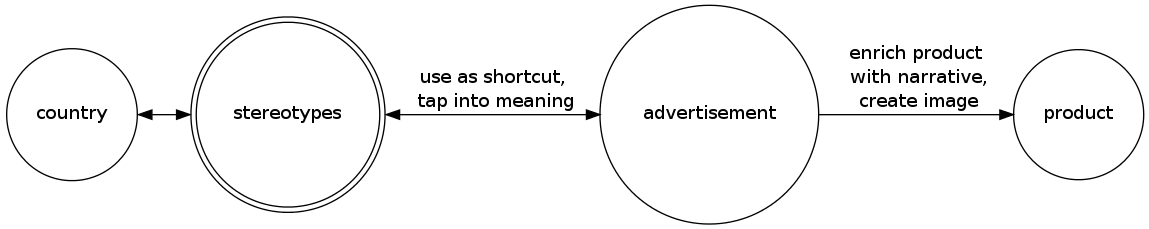
\includegraphics[scale=.25]{concepts.png}
\end{frame}

% \subsection{Fun fact (?)}
%| Canadian Club | "151 Countries, 1 Rye":http://www.youtube.com/watch?v=3H9wDdRk0vs | various | - |

\end{document}
